\documentclass[border=10pt]{standalone}

\usepackage{tikz}
\usepackage{tikzsymbols}
\usetikzlibrary{calc,patterns,shapes.geometric}

\def\centerarc[#1](#2)(#3:#4:#5){\draw[#1] ($(#2)+({#5*cos(#3)},{#5*sin(#3)})$) arc (#3:#4:#5);}

\begin{document}
	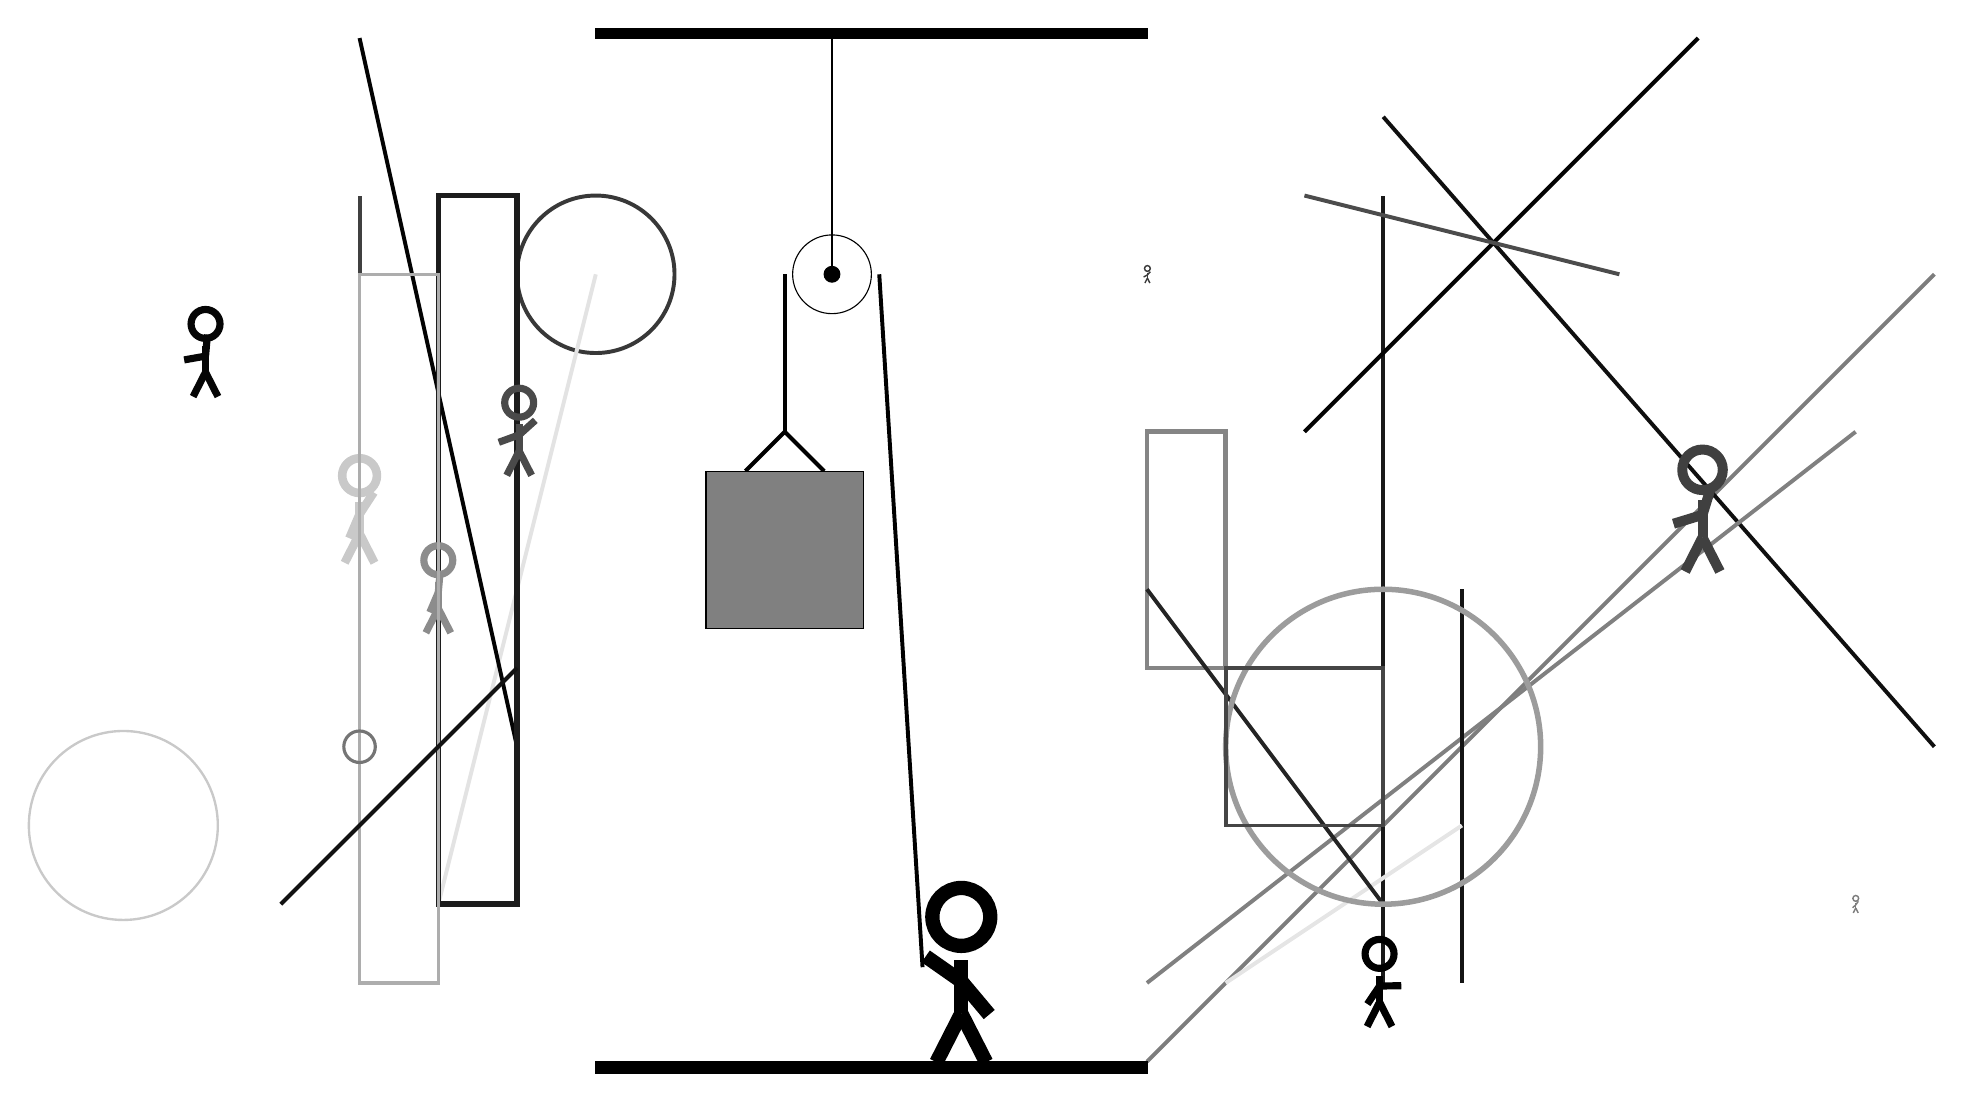
\begin{tikzpicture}
		%%%%% START %%%%%
		
		\draw[fill=black] (-2, 10) rectangle (5, 10.125);
		
		\draw (1, 7) circle (0.5);
		\draw[fill=black] (1, 7) circle (0.1);
		\draw (1, 10) -- (1, 7);
		
		\draw[line width=0.5mm] (-0.1, 4.5) -- (0.4, 5.0) -- (0.9, 4.5);
		\draw[fill=black!50] (-0.6, 4.5) rectangle (1.4, 2.5);
		
		\draw[line width=0.5mm] (0.4, 7) -- (0.4, 5.0);
		\centerarc[line width=0.5mm](1, 7)(0:180:0.6);
		\draw[line width=0.5mm](1.6, 7) -- (2.15, -1.8);
		
		\draw [line width=0.5mm, color=black!78](-2, 7) circle (1.0);
		
		\draw[line width=0.5mm, color=black!51](5, -3) -- (15, 7);
		\draw[line width=0.5mm, color=black!90](8, -2) -- (8, 8);
		\draw[line width=0.5mm, color=black!11](-4, -1) -- (-2, 7);
		\draw[line width=0.5mm, color=black!99](-5, 10) -- (-3, 1);
		\node[line width=0.2mm, color=black!21] at (-5, 4) {\Strichmaxerl[6][67][57]};
		\draw[line width=0.5mm, color=black!94](8, 9) -- (15, 1);
		
		\node[line width=0.6mm, color=black!51] at (14, -1) {\Strichmaxerl[1][43][54]};
		\draw[line width=0.5mm, color=black!50](5, -2) -- (14, 5);
		
		\draw[line width=0.5mm, color=black!75](-5, 7) -- (-5, 8);
		\draw[line width=0.7mm, color=black!89] (-4, -1) rectangle (-3, 8);
		\node[line width=0.4mm, color=black!98] at (-7, 6) {\Strichmaxerl[5][10][85]};
		\draw[line width=0.5mm, color=black!92](9, 3) -- (9, -2);
		\node[line width=0.3mm, color=black!45] at (-4, 3) {\Strichmaxerl[5][67][85]};
		\node[line width=0.2mm, color=black!75] at (12, 4) {\Strichmaxerl[7][17][73]};
		\node[line width=0.5mm, color=black!77] at (5, 7) {\Strichmaxerl[1][29][48]};
		
		\draw [line width=0.3mm, color=black!21](-8, 0) circle (1.2);
		\draw[line width=0.4mm, color=black!32] (-4, -2) rectangle (-5, 7);
		\draw[line width=0.5mm, color=black!10](6, -2) -- (9, 0);
		
		\draw[line width=0.5mm, color=black!99](7, 5) -- (12, 10);
		\draw [line width=0.4mm, color=black!54](-5, 1) circle (0.2);
		
		\draw[line width=0.5mm, color=black!93](-3, 2) -- (-6, -1);
		\draw[line width=0.6mm, color=black!48] (6, 5) rectangle (5, 2);
		\draw[line width=0.5mm, color=black!86](8, -1) -- (5, 3);
		\draw[line width=0.5mm, color=black!70](7, 8) -- (11, 7);
		
		\node[line width=0.4mm, color=black!100] at (8, -2) {\Strichmaxerl[5][56][1]};
		\draw [line width=0.7mm, color=black!39](8, 1) circle (2.0);
		\node[line width=0.6mm, color=black!71] at (-3, 5) {\Strichmaxerl[5][20][42]};
		\draw[line width=0.5mm, color=black!73] (6, 2) rectangle (8, 0);
		
		
		\node at (2.6, -1.9) {\Strichmaxerl[10][-35][-50]};
		
		\draw[fill=black] (-2, -3) rectangle (5, -3.15);
		
		%%%%% END %%%%%
	\end{tikzpicture}
\end{document}